\documentclass[12pt,a4paper,oneside]{report}

%==================== GOI THU VIEN ====================
\usepackage{fontspec}
\usepackage[fontsize=13pt]{fontsize}
\usepackage{geometry}
\usepackage{graphicx}
\usepackage{xcolor}
\usepackage{setspace}
\usepackage{titlesec}
\usepackage{tocloft}
\usepackage{enumitem}
\usepackage{booktabs}
\usepackage{array}
\usepackage{longtable}
\usepackage{tikz}
\usepackage{caption}
\usepackage{fancyhdr}
\usepackage[hidelinks]{hyperref}
\usetikzlibrary{arrows.meta,positioning,shapes.geometric,calc,fit,backgrounds}

%==================== TRANG & FONT ====================
\geometry{a4paper,left=3cm,right=2cm,top=2cm,bottom=2cm}
\setmainfont{Times New Roman}
\onehalfspacing
\setlength{\parindent}{1cm}
\setlength{\parskip}{1pt}
\setlength{\textfloatsep}{12pt plus 2pt minus 3pt}
\setlength{\intextsep}{12pt plus 2pt minus 3pt}
\setlength{\abovecaptionskip}{7pt}

% tieng Viet khong ngat tu
\hyphenpenalty=10000
\exhyphenpenalty=10000
\tolerance=2500
\emergencystretch=3em

\definecolor{docdo}{RGB}{204,0,0}
\definecolor{xanhkv}{RGB}{16,54,110}
\definecolor{xamnhat}{RGB}{242,244,247}
\definecolor{xamvien}{RGB}{170,178,189}
\definecolor{cotbieudo}{RGB}{42,92,168}

%==================== DINH DANG DE MUC I. / a. ====================
\renewcommand{\thesection}{\Roman{section}}
\renewcommand{\thesubsection}{\alph{subsection}}
\renewcommand{\thesubsubsection}{\arabic{subsubsection}}

\titleformat{\section}{\normalfont\bfseries\large}{\thesection.}{0.6em}{}
\titlespacing*{\section}{0pt}{18pt}{10pt}
\titleformat{\subsection}{\normalfont\bfseries}{\thesubsection.}{0.6em}{}
\titlespacing*{\subsection}{0pt}{14pt}{8pt}
\titleformat{\subsubsection}{\normalfont\bfseries\itshape}{\thesubsubsection.}{0.5em}{}
\titlespacing*{\subsubsection}{0pt}{12pt}{6pt}

%==================== MUC LUC ====================
\renewcommand{\contentsname}{MỤC LỤC}
\renewcommand{\cfttoctitlefont}{\hfill\normalfont\Large\MakeUppercase}
\renewcommand{\cftaftertoctitle}{\hfill}
\renewcommand{\cftsecfont}{\bfseries}
\renewcommand{\cftsecaftersnum}{.}
\renewcommand{\cftsubsecaftersnum}{.}
\setlength{\cftbeforesecskip}{6pt}

%==================== CAPTION HINH / BANG ====================
\renewcommand{\figurename}{Hình}
\renewcommand{\tablename}{Bảng}
\captionsetup{font=small,labelfont=bf,labelsep=period,justification=centering}
\renewcommand{\thefigure}{\arabic{figure}}
\renewcommand{\thetable}{\arabic{table}}

%==================== HEADER / FOOTER ====================
\pagestyle{fancy}
\fancyhf{}
\fancyfoot[C]{\small\thepage}
\renewcommand{\headrulewidth}{0pt}

%==================== MACRO RIENG ====================
% dong ke bang dau cham cho trang danh gia
\newcommand{\dongcham}{\par\vspace{1.15em}\noindent\dotfill\par}

% khung ghi chu nhe
\newenvironment{khungy}
  {\par\vspace{6pt}\begin{list}{}{\leftmargin=1cm \rightmargin=0.4cm}\item[]\itshape}
  {\end{list}\vspace{4pt}}

\begin{document}

%==================== TRANG BIA ====================
\thispagestyle{empty}
\begin{center}
\setstretch{1.15}

{\fontsize{14}{18}\selectfont\bfseries ĐẠI HỌC QUỐC GIA HÀ NỘI}\\[6pt]
{\fontsize{14}{18}\selectfont\bfseries TRƯỜNG ĐẠI HỌC CÔNG NGHỆ}\\[10pt]

{\fontsize{13}{16}\selectfont \makebox[7.4cm]{\leaders\hbox to 4.4pt{\hss-\hss}\hfill}}\\[14pt]


\includegraphics[width=2.9cm]{hinh/logo-uet.png}\\[20pt]

{\fontsize{34}{40}\selectfont BÁO CÁO THỰC TẬP}\\[14pt]

{\fontsize{17}{22}\selectfont NGÀNH: \textcolor{docdo}{CÔNG NGHỆ THÔNG TIN}}\\[20pt]

{\fontsize{17}{23}\selectfont \underline{ĐỀ TÀI}: \textcolor{docdo}{PHÁT TRIỂN VÀ TỐI ƯU TÍNH NĂNG\\ CHO HỆ THỐNG QUẢN LÝ KHÁCH SẠN\\ KIOTVIET HOTEL}}\\[26pt]

{\fontsize{13}{18}\selectfont Cán bộ hướng dẫn: \textcolor{docdo}{Trần Mạnh Cường}}\\[18pt]

\end{center}

\hfill
\begin{minipage}{0.62\textwidth}
\setstretch{1.25}
\fontsize{13}{18}\selectfont
\textbf{Giảng viên đánh giá:} \textcolor{docdo}{[chờ bổ sung]}\\
\textbf{Sinh viên:} \textcolor{docdo}{Trần Quang Thành}\\
\textbf{Mã sinh viên:} \textcolor{docdo}{23020155}\\
\textbf{Lớp:} \textcolor{docdo}{K68I-IT2}
\end{minipage}

\vfill
\begin{center}
{\fontsize{14}{18}\selectfont\bfseries Hà Nội, \textcolor{docdo}{tháng 9 năm 2026}}
\end{center}
\vspace{6pt}
\clearpage

%==================== MUC LUC ====================
\tableofcontents
\thispagestyle{empty}
\clearpage

%==================== LOI CAM ON ====================
\thispagestyle{empty}
\begin{center}
{\fontsize{17}{22}\selectfont LỜI CẢM ƠN}
\end{center}
\vspace{20pt}

Thời gian làm việc tại KiotViet là quãng thời gian quý báu giúp em tích lũy được nhiều kinh nghiệm thực tế trước khi hoàn thành chương trình đại học. Em xin cảm ơn công ty KiotViet đã tạo điều kiện cho em được tiếp xúc, học hỏi và làm việc trong một môi trường chuyên nghiệp, năng động. Em xin gửi lời cảm ơn chân thành tới anh Nguyễn Mạnh Cường, người trực tiếp hướng dẫn em tại công ty. Anh luôn gợi mở và hướng dẫn em cách tự tìm hiểu bản chất của vấn đề thay vì đưa ra lời giải ngay. Những lần anh yêu cầu em tự giải thích và kiểm tra lại thay đổi trước khi đưa lên hệ thống đã giúp em hình thành thói quen cẩn trọng và có trách nhiệm hơn với công việc của mình.

Em cũng xin cảm ơn các anh chị trong nhóm phát triển sản phẩm khách sạn. Cảm ơn các anh chị đã luôn nhiệt tình hỗ trợ một người mới, kiên nhẫn chỉ ra những điểm chưa tối ưu trong mã nguồn và sẵn sàng chia sẻ kinh nghiệm thực tế giúp em tiến bộ nhanh hơn trong công việc.

Em xin cảm ơn các thầy cô Trường Đại học Công nghệ, Đại học Quốc gia Hà Nội. Những kiến thức nền tảng về cơ sở dữ liệu, cấu trúc dữ liệu và giải thuật cùng công nghệ phần mềm được học tại trường đã giúp em tiếp cận công việc thực tế một cách thuận lợi và vững vàng hơn.

Cuối cùng, em xin gửi lời cảm ơn sâu sắc tới thầy Trần Mạnh Cường vì đã dành thời gian định hướng và hướng dẫn cho em hoàn thành học phần thực tập doanh nghiệp này. Báo cáo khó tránh khỏi những thiếu sót, em rất mong nhận được những ý kiến đóng góp của thầy để báo cáo được hoàn thiện hơn.

Em xin chân thành cảm ơn!

\vspace{24pt}
\begin{flushright}
\begin{minipage}{0.5\textwidth}
\centering
Hà Nội, tháng 9 năm 2026\\
\textit{Sinh viên}\\[26pt]
\textbf{Trần Quang Thành}
\end{minipage}
\end{flushright}

\clearpage


\setcounter{page}{1}
\section{Giới thiệu chung}

\subsection{Giới thiệu công ty}

KiotViet là thương hiệu phần mềm quản lý bán hàng do Công ty Cổ phần Công nghệ Citigo phát triển, ra đời với mục tiêu giúp những cửa hàng vừa và nhỏ ở Việt Nam quản lý việc bán hàng bằng phần mềm thay vì bằng sổ tay. Từ nhóm khách hàng ban đầu là các cửa hàng bán lẻ, công ty mở rộng dần sang nhà hàng, quán cà phê, cửa hàng làm đẹp và khách sạn; mỗi ngành có cách vận hành riêng nên được tách thành những dòng sản phẩm khác nhau dùng chung phần nền bên dưới.

Em thực tập tại nhóm phát triển sản phẩm cho ngành khách sạn. Sản phẩm phục vụ khách sạn, nhà nghỉ, homestay và resort, với người dùng cuối là lễ tân, thu ngân, buồng phòng, kế toán và chủ cơ sở lưu trú. Điểm đáng chú ý là sản phẩm không chỉ chạy ở Việt Nam mà còn được dùng ở một số nước khác trong khu vực, nên phần mềm phải nói được nhiều thứ tiếng và tính toán đúng theo múi giờ, đơn vị tiền tệ của từng nơi.

\subsection{Giới thiệu công việc}

Em tham gia nhóm với vai trò thực tập sinh phát triển phần mềm, làm cả phần giao diện và phần xử lý phía máy chủ, từ ngày 12 tháng 3 năm 2026 đến ngày 7 tháng 9 năm 2026.

Ngày đầu em hơi choáng. Sản phẩm không nằm trong một kho mã duy nhất mà chia thành chín kho mã riêng: màn hình cho lễ tân, màn hình cho người quản lý, dịch vụ xử lý đơn đặt phòng, dịch vụ sinh báo cáo, dịch vụ xuất nhập tệp dữ liệu, phần giao tiếp với ứng dụng di động và phần nền dùng chung. Tổng cộng có hàng trăm nghìn dòng mã đã tồn tại từ trước, do rất nhiều người viết qua nhiều năm. Em mất gần hai tuần đầu chỉ để trả lời được câu hỏi đơn giản nhất: khi lễ tân bấm một nút trên màn hình thì dữ liệu chạy qua những đâu.

Công việc của em chia thành bốn nhóm: sửa lỗi được báo về từ khách hàng đang dùng thật, làm tính năng mới theo yêu cầu, tối ưu hiệu năng ở những chỗ làm hệ thống chậm hoặc chặn nhau, và tham gia dựng phần quản lý phiên bản mới.

\begin{table}[htbp]
\centering
\caption{Tóm tắt đóng góp trong kỳ thực tập}
\label{bang:dongghop}
\small
\setstretch{1.1}
\begin{tabular}{@{}>{\raggedright\arraybackslash}p{7.6cm}r@{}}
\toprule
\textbf{Hạng mục} & \textbf{Số liệu} \\
\midrule
Thời gian thực tập & 12/03/2026 đến 07/09/2026 \\
Số kho mã đã tham gia & 9 \\
Số lần ghi mã, không tính lần gộp nhánh & 698 \\
Số đầu việc khác nhau đã xử lý & 342 \\
Số phiếu công việc đã hoàn thành & 173 \\
Số ngày có ghi mã & 99 \\
Số dòng mã thêm mới & 34.994 \\
Số dòng mã xoá bỏ & 10.079 \\
Số lượt sửa tệp & 1.947 \\
Số dòng mã kiểm thử tự động đã viết & 1.919 \\
\bottomrule
\end{tabular}
\end{table}

Bảng \ref{bang:dongghop} tóm tắt phần đóng góp của em, số liệu lấy trực tiếp từ lịch sử mã nguồn. Con số dòng mã đã loại bỏ các tệp bản dịch ngôn ngữ, tệp cấu hình sinh tự động và tệp nhị phân, để phản ánh đúng phần mã do em thực sự viết.

\subsection{Giới thiệu qua bài toán}

Nghe tên thì phần mềm quản lý khách sạn có vẻ đơn giản: khách đến thì nhận phòng, khách đi thì trả phòng và thanh toán. Nhưng khi bắt tay vào làm em mới thấy phần khó không nằm ở chỗ lưu dữ liệu, mà ở chỗ cùng một dữ liệu phải trả lời đúng cho rất nhiều câu hỏi khác nhau, ở nhiều nơi khác nhau, tại nhiều thời điểm khác nhau.

Lấy một ví dụ em gặp thật. Một phòng bị khoá lại để sửa chữa trong ba ngày. Việc này nghe rất nhỏ, nhưng ngay sau đó hàng loạt câu hỏi khác phải đổi câu trả lời: màn hình lễ tân phải không cho đặt phòng đó nữa, lịch phòng phải vẽ ra một khoảng bị chặn, báo cáo công suất phòng phải hiểu rằng phòng này đang không kinh doanh nên không được tính vào mẫu số, và nếu người quản lý xem lại số liệu tháng trước thì phòng đó lại phải được tính bình thường vì lúc ấy nó chưa bị khoá. Một thay đổi ở một chỗ kéo theo hệ quả ở năm sáu chỗ khác, và những chỗ đó do người khác viết từ trước.

Bài toán còn khó thêm vì ba lý do. Thứ nhất, hệ thống đang chạy thật nên không có chuyện làm lại từ đầu. Thứ hai, một khách hàng có thể có nhiều chi nhánh ở nhiều nơi, mỗi nơi một múi giờ và một đồng tiền, nên câu hỏi tưởng dễ như hôm nay bán được bao nhiêu cũng cần định nghĩa rõ hôm nay là theo giờ ở đâu. Thứ ba, phần mềm hiển thị được năm ngôn ngữ, nên mỗi chuỗi chữ, mỗi định dạng ngày và mỗi cách viết số đều phải xử lý cho cả năm. Trong bối cảnh đó, phần việc em nhận không phải là xây một hệ thống mới, mà là bổ sung và làm tốt hơn những phần cụ thể của một hệ thống đang sống.

\section{Yêu cầu bài toán}

\subsection{Miêu tả chi tiết bài toán}

Hệ thống phục vụ ba nhóm người dùng có nhu cầu rất khác nhau, và chính sự khác biệt đó tạo nên phần lớn độ phức tạp trong thiết kế và tối ưu.

Lễ tân và thu ngân làm việc trực tiếp tại quầy vào các khung giờ cao điểm nhận và trả phòng, đòi hỏi thao tác nhanh, quy trình tinh giản và phản hồi tức thì: màn hình phải trả lời ngay phòng nào trống, khách đã thanh toán chưa, số tiền còn thiếu là bao nhiêu. Độ trễ dù chỉ vài giây tại quầy cũng tác động trực tiếp đến sự chờ đợi của khách lưu trú.

Người quản lý và chủ cơ sở quan tâm đến các con số tổng hợp: doanh thu so với kỳ trước, công suất phòng và hiệu quả nguồn khách. Các truy vấn này quét trên tập dữ liệu lớn với yêu cầu khắt khe về tính nhất quán: số liệu giữa báo cáo phân tích và màn hình theo dõi thời gian thực cần đảm bảo tính đồng bộ, không để xảy ra sai lệch. Nhóm thứ ba gồm bộ phận kế toán và buồng phòng với các nghiệp vụ cụ thể như xuất hóa đơn, đối chiếu sổ quỹ, bàn giao ca và cập nhật tình trạng dọn phòng.

Qua quá trình làm việc và tiếp cận hệ thống, em nhận thấy sản phẩm cần đáp ứng một số yêu cầu chính như: số liệu cần đảm bảo tính nhất quán giữa các màn hình nghiệp vụ; quyền thao tác của người dùng phải được kiểm tra ở phía máy chủ, thay vì chỉ ẩn hoặc vô hiệu hóa nút trên giao diện; hệ thống cần hỗ trợ địa phương hóa tốt về ngôn ngữ, múi giờ và tiền tệ; đồng thời cần duy trì hiệu năng ổn định, tránh để các tác vụ xuất nhập dữ liệu lớn gây ảnh hưởng đến thao tác thường nhật của nhân viên tại quầy.

\begin{center}
\vspace{-4pt}
\begin{singlespace}
\begin{tikzpicture}[
  scale=0.88, every node/.append style={transform shape},
  box/.style={draw=xamvien!90!black, fill=xamnhat, rounded corners=3pt, align=center,
              font=\fontsize{8.5pt}{10pt}\selectfont, inner sep=2.5pt},
  nen/.style={draw=xanhkv, fill=white, rounded corners=3pt, align=center,
              font=\fontsize{8.5pt}{10pt}\selectfont, inner sep=2.5pt, thick},
  mui/.style={-{Stealth[length=2.5mm, width=1.6mm]}, draw=xanhkv!90!black, thick}
]

% ===== TẦNG 1: GIAO DIỆN NGƯỜI DÙNG (y = 0) =====
\node[box, text width=6.05cm, minimum height=0.72cm] (fe1) at (3.125, 0)
  {\textbf{\small Màn hình lễ tân}\\[1pt]{\scriptsize Thao tác tại quầy, phản hồi tức thì}};

\node[box, text width=9.25cm, minimum height=0.72cm] (fe2) at (11.25, 0)
  {\textbf{\small Màn hình quản lý}\\[1pt]{\scriptsize Theo dõi vận hành, giám sát và báo cáo}};

% ===== TẦNG 2: DỊCH VỤ NGHIỆP VỤ (y = -1.65) =====
\node[box, text width=2.85cm, minimum height=0.72cm] (sv1) at (1.50, -1.65)
  {\textbf{Dịch vụ đặt phòng}\\[1pt]{\scriptsize Xử lý đặt chỗ}};

\node[box, text width=2.85cm, minimum height=0.72cm] (sv2) at (4.75, -1.65)
  {\textbf{Dịch vụ quản lý}\\[1pt]{\scriptsize Danh mục, giá phòng}};

\node[box, text width=2.85cm, minimum height=0.72cm] (sv3) at (8.00, -1.65)
  {\textbf{Dịch vụ báo cáo}\\[1pt]{\scriptsize Thống kê số liệu}};

\node[box, text width=2.85cm, minimum height=0.72cm] (sv4) at (11.25, -1.65)
  {\textbf{Xuất nhập tệp}\\[1pt]{\scriptsize Xử lý tệp nền}};

\node[box, text width=2.85cm, minimum height=0.72cm] (sv5) at (14.50, -1.65)
  {\textbf{Giao tiếp di động}\\[1pt]{\scriptsize API cho ứng dụng}};

% ===== TẦNG 3: NỀN TẢNG DÙNG CHUNG (y = -3.20) =====
\node[nen, text width=15.70cm, minimum height=0.72cm] (nen) at (8.00, -3.20)
  {\textbf{\small Phần nền dùng chung}\\[1pt]{\scriptsize Thực thể nghiệp vụ, quy tắc phân quyền, cấu hình và thư viện tiện ích}};

% ===== TẦNG 4: CƠ SỞ DỮ LIỆU & LƯU TRỮ (y = -4.65) =====
\node[box, text width=7.65cm, minimum height=0.72cm] (db) at (3.925, -4.65)
  {\textbf{\small SQL Server}\\[1pt]{\scriptsize Lưu trữ có cấu trúc, phân vùng dữ liệu}};

\node[box, text width=7.65cm, minimum height=0.72cm] (redis) at (12.075, -4.65)
  {\textbf{\small Redis}\\[1pt]{\scriptsize Bộ nhớ đệm phân tán, điều phối khoá}};

% ===== MŨI TÊN TẦNG 1 -> TẦNG 2 (Rõ ràng, dài ~0.9cm) =====
\draw[mui] (sv1.north |- fe1.south) -- (sv1.north);
\draw[mui] ([xshift=-0.35cm]sv2.north |- fe1.south) -- ([xshift=-0.35cm]sv2.north);
\draw[mui] ([xshift=0.25cm]fe2.south west) -- ([xshift=0.35cm]sv2.north);
\draw[mui] (sv3.north |- fe2.south) -- (sv3.north);
\draw[mui] (sv4.north |- fe2.south) -- (sv4.north);
\draw[mui] (sv5.north |- fe2.south) -- (sv5.north);

% ===== MŨI TÊN TẦNG 2 -> TẦNG 3 (Dài ~0.85cm, thẳng đứng thanh thoát) =====
\draw[mui] (sv1.south) -- (nen.north -| sv1.south);
\draw[mui] (sv2.south) -- (nen.north -| sv2.south);
\draw[mui] (sv3.south) -- (nen.north -| sv3.south);
\draw[mui] (sv4.south) -- (nen.north -| sv4.south);
\draw[mui] (sv5.south) -- (nen.north -| sv5.south);

% ===== MŨI TÊN TẦNG 3 -> TẦNG 4 (Dài ~0.75cm, thẳng đứng dứt khoát) =====
\draw[mui] (nen.south -| db.north) -- (db.north);
\draw[mui] (nen.south -| redis.north) -- (redis.north);
\end{tikzpicture}
\end{singlespace}
\vspace{-4pt}
\captionof{figure}{Các thành phần chính của hệ thống và quan hệ giữa chúng}
\label{hinh:kientruc}
\vspace{-6pt}
\end{center}

\indent Hình \ref{hinh:kientruc} mô tả kiến trúc phân tầng và sự tương tác giữa các thành phần chính trong hệ thống. Trong quá trình thực tập, em nhận thấy các dịch vụ nghiệp vụ có mối liên kết chặt chẽ với nhau: một thao tác thực tế của người dùng thường đi qua nhiều tầng chức năng, do đó việc đọc hiểu mã nguồn hiện hữu là bước rất quan trọng trước khi bắt tay vào xây dựng tính năng mới.

\subsection{Phần bài toán em trực tiếp giải quyết}

Hệ thống sản phẩm là kết quả xây dựng của cả tập thể qua nhiều giai đoạn. Trong phạm vi thực tập, em được giao đảm nhiệm một số bài toán cụ thể với đầu vào và đầu ra rõ ràng, tập trung vào sáu hướng chính:

\begin{enumerate}[leftmargin=1.2cm, itemsep=2pt, topsep=3pt]
\item Tham gia xây dựng tính năng khóa phòng bảo trì: từ mô hình dữ liệu, quy tắc nghiệp vụ, API phía máy chủ đến giao diện người dùng, bản dịch đa ngôn ngữ và kiểm thử tự động.
\item Bổ sung hai chỉ tiêu thống kê về lượt khách nghỉ qua đêm và tổng số đêm nghỉ-bài toán xử lý khoảng thời gian và băm chuỗi định danh.
\item Tái cấu trúc phân quyền: tách quyền hủy đơn thành hai quyền độc lập, kèm kịch bản chuyển đổi dữ liệu phân quyền hai chiều cho các cơ sở đang hoạt động.
\item Tối ưu hiệu năng: cải tiến các câu truy vấn cơ sở dữ liệu, giải phóng khóa phân tán kịp thời và loại bỏ các phép tính toán lặp dư thừa trên giao diện.
\item Xây dựng các phân hệ cho bản quản lý mới: trang tổng quan (dashboard) với các biểu đồ doanh thu, danh mục phòng và tài liệu hướng dẫn tích hợp kênh bán phòng trực tuyến.
\item Xử lý đa ngôn ngữ và địa phương hóa: bổ sung tiếng Hàn, tiếng Trung, tiếng Lào cho các màn hình, đồng thời chuẩn hóa định dạng ngày tháng, tiền tệ và múi giờ.
\end{enumerate}

\subsection{Công việc của nhóm và công việc của em}

Nhóm phát triển vận hành theo mô hình đa chức năng: chuyên viên phân tích nghiệp vụ đặc tả yêu cầu; thiết kế trải nghiệm dựng giao diện; lập trình viên hiện thực logic; chuyên viên kiểm thử (QA) kiểm tra chất lượng trước phát hành; hỗ trợ kỹ thuật tiếp nhận phản hồi từ khách hàng; và trưởng nhóm điều phối, rà soát mã nguồn cùng tiến độ.

Trong cấu trúc đó, em tham gia với vai trò thực tập sinh phát triển phần mềm. Quy trình xử lý một phiếu công việc bắt đầu từ việc tiếp nhận yêu cầu, trao đổi làm rõ trường hợp biên, đọc mã nguồn hiện hữu để xác định phạm vi ảnh hưởng, viết mã, tự kiểm thử, bổ sung kiểm thử tự động cho logic quan trọng, gửi rà soát mã nguồn (code review) và phối hợp với bộ phận kiểm thử đến khi nghiệm thu hoàn tất.

Một bài học làm thay đổi nhận thức nghề nghiệp của em: nhiệm vụ thực sự của người phát triển không chỉ là làm cho tính năng chạy được, mà phải đảm bảo nó hoạt động chuẩn xác mà không gây ảnh hưởng tiêu cực đến bất kỳ hành vi nghiệp vụ nào đang vận hành ổn định trên hệ thống.

\section{Tóm tắt lý thuyết, giải pháp, thuật toán}

\subsection{Các lý thuyết và giải pháp liên quan}

Trong quá trình thực tập, em đã trực tiếp vận dụng các nền tảng của khoa học máy tính và nguyên lý thiết kế phần mềm vào quá trình phân tích, xây dựng và cải tiến hệ thống. Những kiến thức này được gắn với các bài toán thực tế và các giải pháp kỹ thuật được trình bày trong những phần tiếp theo.

\begin{itemize}[leftmargin=1.2cm, itemsep=3pt, topsep=3pt]
\item \textbf{Kiến trúc phân tầng và nguyên tắc đảo ngược phụ thuộc:} Hệ thống được tổ chức thành các tầng với trách nhiệm rõ ràng theo nguyên lý kiến trúc sạch (Clean Architecture) [1]: tầng giao diện xử lý tương tác với người dùng, tầng ứng dụng và nghiệp vụ xử lý các quy tắc của hệ thống, còn tầng hạ tầng đảm nhiệm việc làm việc với cơ sở dữ liệu và các thành phần bên ngoài. Các tầng nghiệp vụ cốt lõi được thiết kế để không phụ thuộc trực tiếp vào giao diện hay công nghệ lưu trữ cụ thể. Nhờ đó, các quy tắc nghiệp vụ quan trọng được tập trung và quản lý thống nhất, đồng thời có thể được sử dụng lại ở nhiều chức năng khác nhau mà không phải sao chép hoặc viết lại cùng một logic.

\item \textbf{Phân tách lệnh và truy vấn (CQRS):} Hệ thống áp dụng mô hình phân tách lệnh và truy vấn (CQRS) [4] để tách riêng các thao tác làm thay đổi dữ liệu (Command) với các thao tác chỉ đọc và truy xuất dữ liệu (Query). Với các nghiệp vụ như đặt phòng, thay vì thay đổi trực tiếp trạng thái của bản ghi, hệ thống xử lý thông qua các lệnh thể hiện rõ mục đích của nghiệp vụ. Cách tiếp cận này giúp dễ dàng theo dõi và lưu lại lịch sử thay đổi, đồng thời cho phép phần xử lý dữ liệu đọc được tối ưu riêng cho các chức năng như báo cáo và thống kê mà không ảnh hưởng đến quá trình ghi dữ liệu.

\item \textbf{Chi phí của tầng trừu tượng khi truy cập dữ liệu (ORM Overhead):} Các công cụ ánh xạ đối tượng-quan hệ (ORM) như Entity Framework [6] giúp lập trình viên thao tác với cơ sở dữ liệu thông qua ngôn ngữ bậc cao. Tuy nhiên, nếu sử dụng không phù hợp, tầng trừu tượng này có thể sinh ra các câu truy vấn phức tạp, nạp thừa dữ liệu qua mạng (over-fetching) hoặc dẫn đến hiện tượng bùng nổ tích Descartes khi nối nhiều bảng quan hệ. Tại các tác vụ xử lý lượng bản ghi lớn, việc xem xét kế hoạch thực thi (Execution Plan) và cơ chế khóa [7] kết hợp sử dụng các câu truy vấn định hướng (Projection Queries) là yếu tố quan trọng để đảm bảo hiệu năng.

\item \textbf{Khóa phân tán và quản lý vòng đời khóa (Distributed Lock with TTL):} Khi nhiều tiến trình cùng truy cập và cập nhật tài nguyên dùng chung, khóa phân tán trên Redis hỗ trợ xử lý tuần tự và hạn chế xung đột tài nguyên [8]. Việc thiết lập thời gian sống (TTL) cho khóa là điều cần thiết để giảm nguy cơ khóa bị giữ vô thời hạn (stale lock) trong trường hợp một tiến trình gặp sự cố bất thường trước khi kịp giải phóng khóa.

\item \textbf{Cơ chế phát hiện thay đổi trên giao diện (Change Detection):} Trong Angular, quá trình phát hiện thay đổi có thể khiến các biểu thức trong template được đánh giá lại qua nhiều chu kỳ cập nhật giao diện [5]. Do đó, việc gọi trực tiếp các hàm tính toán phức tạp hoặc quét mảng trong template có thể bị kích hoạt lặp đi lặp lại, gây sụt giảm khung hình và làm giao diện phản hồi chậm chạp.

\item \textbf{Thuật toán gộp khoảng và tính giao thời gian (Interval Merging):} Cho một tập các khoảng thời gian có khả năng chồng lấn $I = \{[s_i, e_i]\}$ [3], thuật toán tiến hành sắp xếp theo mốc bắt đầu với độ phức tạp $O(k \log k)$, sau đó duyệt tuần tự trong $O(k)$ để hợp nhất các khoảng có phần giao nhau thành các khoảng liên tục không chồng lấn. Từ các khoảng đã gộp, hệ thống tính toán phần giao thực tế với một khung thời gian quan sát $[T_{\text{start}}, T_{\text{end}}]$ cho trước.

\item \textbf{Hàm băm một chiều bảo vệ dữ liệu định danh (One-way Hashing):} Nhằm tuân thủ các quy chuẩn bảo mật và an toàn thông tin cá nhân (PII), dữ liệu định danh của khách lưu trú được chuyển thành giá trị băm có độ dài cố định bằng hàm băm một chiều. Kỹ thuật này cho phép hệ thống đối chiếu và gom nhóm khách hàng dựa trên giá trị định danh mà không cần sử dụng trực tiếp thông tin gốc trên phân hệ báo cáo.

\item \textbf{Chuẩn hóa chuỗi văn bản tìm kiếm đa ngôn ngữ (Unicode Normalization):} Xử lý tìm kiếm trong môi trường đa ngôn ngữ đòi hỏi chuẩn hóa cả chuỗi người dùng nhập lẫn dữ liệu nguồn về dạng chuẩn (như NFC). Đồng thời, thuật toán sử dụng các thuộc tính ký tự Unicode (\texttt{\textbackslash p\{L\}}, \texttt{\textbackslash p\{N\}}) theo chuẩn Unicode [9] thay cho các biểu thức chính quy thuần ASCII, nhằm bảo toàn trọn vẹn dấu tiếng Việt và các hệ ký tự tượng hình như tiếng Hàn và tiếng Trung.
\end{itemize}

\subsection{Cách giải quyết của em}

\subsubsection{Tính năng khóa phòng: xử lý thay đổi trạng thái}

Tính năng khóa phòng phục vụ nhu cầu tạm ngừng kinh doanh một hoặc nhiều phòng trong một khoảng thời gian xác định kèm lý do bảo trì hoặc sửa chữa. Vấn đề phức tạp nhất xuất hiện ở thao tác chỉnh sửa: người dùng mở một lượt khóa hiện có, sau đó có thể đồng thời thêm phòng mới, loại bỏ phòng cũ, thay đổi khung thời gian bắt đầu/kết thúc và cập nhật lại nội dung lý do.

Phương án đơn giản nhất có thể nghĩ tới là xóa sạch toàn bộ lượt khóa cũ rồi tạo lại lượt mới từ đầu. Phương án này dễ lập trình nhưng bộc lộ hai nhược điểm: lịch sử biến động phòng bị xóa trắng khiến ban quản lý khó truy vết những thay đổi đã thực hiện; đồng thời, các phòng không hề bị thay đổi cũng phải trải qua chu kỳ hủy và tạo lại, gây ra các biến động trạng thái dư thừa và làm tăng nguy cơ xung đột khóa với các đơn đặt phòng khác đang diễn ra.

Để xử lý vấn đề này, em so sánh trạng thái phòng trước và sau khi chỉnh sửa để xác định chính xác những thay đổi thực tế cần xử lý. Cụ thể, gọi $R_{\text{old}}$ là tập phòng đang khóa và $R_{\text{new}}$ là tập phòng sau chỉnh sửa: các phòng thuộc $R_{\text{new}} \setminus R_{\text{old}}$ sinh lệnh giữ phòng mới; các phòng thuộc $R_{\text{old}} \setminus R_{\text{new}}$ sinh lệnh giải phóng; nếu khung thời gian thay đổi thì sinh lệnh điều chỉnh thời gian; và nếu chỉ sửa đổi lý do thì chỉ phát sinh lệnh cập nhật ghi chú. Thành phần xử lý sai khác này được thiết kế độc lập với cơ sở dữ liệu, giúp thuận tiện cho việc viết kiểm thử tự động với các kịch bản tổ hợp.

\begin{figure}[htbp]
\centering
\begin{tikzpicture}[
  hop/.style={draw=xamvien, fill=xamnhat, rounded corners=2pt, align=center,
              font=\small, inner sep=4pt},
  lenh/.style={draw=xanhkv, fill=white, rounded corners=2pt, align=left,
               font=\scriptsize, inner sep=4pt, text width=4.2cm},
  mui/.style={-{Stealth[length=2mm]}, draw=xamvien, thick}
]
\node[hop, text width=3.6cm, minimum height=1.1cm] (cu) at (0,0)
  {\textbf{Trạng thái hiện lưu}\\[1pt]{\scriptsize Danh sách phòng và khoảng thời gian}};
\node[hop, text width=3.6cm, minimum height=1.1cm] (moi) at (0,-2.2)
  {\textbf{Trạng thái gửi lên}\\[1pt]{\scriptsize Dữ liệu sau khi người dùng sửa}};
\node[hop, text width=2.6cm, minimum height=1.5cm, fill=white, draw=xanhkv, thick] (ss) at (5.0,-1.1)
  {\textbf{So sánh sai khác}\\[2pt]{\scriptsize Xác định biến động thực tế}};

\node[lenh] (l1) at (10.1,0.6) {Phòng mới bổ sung\\ $\rightarrow$ Lệnh giữ phòng};
\node[lenh] (l2) at (10.1,-0.75) {Phòng bị loại bỏ\\ $\rightarrow$ Lệnh giải phóng giữ phòng};
\node[lenh] (l3) at (10.1,-2.1) {Khung thời gian thay đổi\\ $\rightarrow$ Lệnh điều chỉnh thời gian};
\node[lenh] (l4) at (10.1,-3.45) {Chỉ lý do thay đổi\\ $\rightarrow$ Lệnh cập nhật ghi chú};

\draw[mui] (cu.east) -- (ss.west);
\draw[mui] (moi.east) -- (ss.west);
\draw[mui] (ss.east) -- (l1.west);
\draw[mui] (ss.east) -- (l2.west);
\draw[mui] (ss.east) -- (l3.west);
\draw[mui] (ss.east) -- (l4.west);
\end{tikzpicture}
\caption{Chỉ sinh lệnh cho phần thực sự thay đổi thay vì huỷ và tạo lại toàn bộ}
\label{hinh:sinhlenh}
\end{figure}

\indent Hình \ref{hinh:sinhlenh} minh họa trực quan luồng phát sinh lệnh có chọn lọc. Toàn bộ các quy tắc kiểm tra tính hợp lệ của dữ liệu đầu vào cũng được tập trung tại một đầu mối duy nhất: loại khóa hợp lệ, giới hạn độ dài lý do, bắt buộc chọn ít nhất một phòng, không cho phép chọn trùng lặp và thời điểm kết thúc luôn phải sau thời điểm bắt đầu. Việc gom cụm quy tắc này bảo đảm thông báo lỗi đồng nhất trên toàn hệ thống.

Ở tầng giao diện, em xây dựng hộp thoại thao tác tích hợp vào sơ đồ lịch phòng và bổ sung cơ chế kiểm tra chặn khi đặt phòng. Đặc biệt, sau khi hoàn thành tính năng, em chủ động phân tích tác động dây chuyền và phát hiện các công thức tính tỷ lệ công suất phòng đang tính cả phòng bị khóa vào số phòng khả dụng để bán. Điều này khiến tỷ lệ lấp đầy hiển thị thấp hơn thực tế, làm sai lệch đánh giá hiệu quả kinh doanh của cơ sở. Em đã chủ động trao đổi và điều chỉnh lại công thức để loại trừ các phòng đang khóa bảo trì ra khỏi mẫu số tính công suất, giúp số liệu thống kê phản ánh chính xác thực tế vận hành.

\subsubsection{Thống kê lượt khách nghỉ qua đêm và tổng số đêm nghỉ}

Yêu cầu bài toán là bổ sung hai chỉ tiêu thống kê quan trọng vào báo cáo phòng trong một khoảng thời gian tùy chọn. Khi phân tích yêu cầu, em nhận thấy phần tính toán cần xử lý ba vấn đề chính:

\textbf{1. Xử lý các khoảng lưu trú chồng lấn:} Một khách hàng có thể có nhiều bản ghi lưu trú nối tiếp hoặc chồng lấn nhau trong kỳ do đổi phòng hoặc gia hạn phòng. Nếu cộng dồn số đêm của từng bản ghi, các ngày trùng lặp sẽ bị tính nhiều lần làm phồng số liệu. Em áp dụng thuật toán gộp khoảng [3]: sắp xếp toàn bộ các bản ghi của cùng một khách theo thời điểm nhận phòng, sau đó duyệt tuần tự để hợp nhất các khoảng có phần giao nhau thành các khoảng lưu trú liên tục duy nhất.

\textbf{2. Cắt khoảng theo biên kỳ báo cáo:} Một lượt lưu trú có thể bắt đầu trước hoặc kết thúc sau khoảng thời gian đang xét. Em xác định riêng quy tắc tính toán cho từng chỉ tiêu: số lượt khách chỉ được ghi nhận khi thời điểm nhận phòng nằm trong kỳ báo cáo (vì lượt là một sự kiện phát sinh); trong khi tổng số đêm nghỉ được tính bằng độ dài phần giao thực tế giữa các khoảng lưu trú đã gộp với khung thời gian báo cáo.

\begin{figure}[htbp]
\centering
\begin{tikzpicture}[font=\small]
\draw[->, thick, draw=xamvien] (0,0) -- (11.9,0) node[right,font=\scriptsize]{thời gian};
\foreach \x/\l in {1/1,3/3,5/5,7/7,9/9,11/11} {
  \draw[draw=xamvien] (\x,-0.1) -- (\x,0.1);
  \node[font=\scriptsize, below=1pt] at (\x,-0.1) {ngày \l};
}
\fill[xanhkv, opacity=0.08] (3,-0.55) rectangle (9,4.3);
\draw[dashed, thick, draw=xanhkv] (3,-0.55) -- (3,4.3);
\draw[dashed, thick, draw=xanhkv] (9,-0.55) -- (9,4.3);
\node[font=\scriptsize\bfseries, text=xanhkv] at (6,4.05) {kỳ báo cáo đang xem};

\node[font=\scriptsize, anchor=east] at (-0.15,3.4) {bản ghi 1};
\draw[line width=3.5pt, draw=xamvien] (1,3.4) -- (4,3.4);
\node[font=\scriptsize, anchor=east] at (-0.15,2.85) {bản ghi 2};
\draw[line width=3.5pt, draw=xamvien] (3.4,2.85) -- (6,2.85);
\node[font=\scriptsize, anchor=east] at (-0.15,2.3) {bản ghi 3};
\draw[line width=3.5pt, draw=xamvien] (7,2.3) -- (11,2.3);

\node[font=\scriptsize, anchor=east] at (-0.15,1.45) {sau khi gộp};
\draw[line width=3.5pt, draw=xanhkv] (1,1.45) -- (6,1.45);
\draw[line width=3.5pt, draw=xanhkv] (7,1.45) -- (11,1.45);

\node[font=\scriptsize, anchor=east] at (-0.15,0.75) {phần được tính};
\draw[line width=3.5pt, draw=xanhkv] (3,0.75) -- (6,0.75);
\draw[line width=3.5pt, draw=xanhkv] (7,0.75) -- (9,0.75);
\end{tikzpicture}
\caption{Gộp các khoảng lưu trú chồng lấn rồi cắt theo biên của kỳ báo cáo}
\label{hinh:gopkhoang}
\end{figure}

\indent Hình \ref{hinh:gopkhoang} mô tả hai bước xử lý: ba bản ghi ban đầu sau khi hợp nhất tạo thành hai khoảng rời rạc; khi đối chiếu theo khung báo cáo, các phần nằm ngoài khoảng thời gian báo cáo được loại bỏ. Bản ghi 1 bắt đầu trước kỳ nên không tính vào số lượt, nhưng các đêm nằm trong kỳ vẫn được tính đầy đủ vào tổng số đêm nghỉ.

\textbf{3. Xử lý trường hợp định danh rỗng:} Khách hàng được nhận diện thông qua giá trị băm của thông tin định danh cá nhân. Trong quá trình kiểm tra thực tế, em phát hiện một vấn đề nghiệp vụ: đối với những khách vãng lai hoặc khách thuê theo giờ không khai báo giấy tờ tùy thân, chuỗi định danh ban đầu là chuỗi rỗng. Khi đi qua hàm băm, chuỗi rỗng luôn sinh ra cùng một giá trị băm cố định. Nếu gom nhóm đơn thuần theo giá trị băm này, toàn bộ khách không khai báo giấy tờ trong suốt kỳ báo cáo sẽ bị gộp thành một người duy nhất, dẫn đến số lượt khách hiển thị bị sai lệch nghiêm trọng. Để khắc phục, hệ thống phân biệt trường hợp không có định danh và quản lý các lượt lưu trú này dựa trên mã đặt phòng (booking code) kết hợp thời gian lưu trú cụ thể, nhờ đó mỗi lượt khách chưa khai báo giấy tờ vẫn được tính toán độc lập và chính xác theo đúng nghiệp vụ.

Toàn bộ logic tính toán được đóng gói thành một lớp thuần túy độc lập với cơ sở dữ liệu, cho phép thiết lập bộ kiểm thử bao phủ các tình huống biên phức tạp. Trong đó, em bổ sung trường hợp kiểm thử kiểm tra tính chất nhất quán của thuật toán: tổng kết quả tính toán của hai khoảng thời gian liên tiếp ghép lại phải bằng đúng kết quả khi tính một lần trên toàn bộ khoảng thời gian gộp.

\subsubsection{Tối ưu quá trình xuất dữ liệu và xử lý các vấn đề về hiệu năng}

Chức năng xuất tệp sổ quỹ gặp tình trạng chậm khi dữ liệu lớn. Phân tích mã nguồn cho thấy phần lấy tên phòng được xây dựng bằng nhiều biểu thức lồng nhau, thực hiện phép nối trên nhiều bảng và lọc trùng lặp qua nhiều bước. Tuy nhiên, điểm nghẽn lớn nhất nằm ở thuật toán xử lý dữ liệu sau khi nạp: mã nguồn cũ duyệt qua từng dòng của tệp và quét tuần tự toàn bộ danh sách phòng để tìm kiếm tên tương ứng. Với tệp $n$ dòng và danh sách phòng $m$ phần tử, số phép so sánh có độ phức tạp $O(n \times m)$, gây độ trễ đáng kể khi xuất hàng nghìn bản ghi.

Em tái cấu trúc thuật toán theo ba bước: kiểm tra sớm nếu không có dữ liệu cần xuất thì dừng ngay; chuyển đổi chuỗi biểu thức phức tạp thành một câu lệnh truy vấn chuẩn hóa duy nhất ở tầng cơ sở dữ liệu để lấy đủ thông tin cần thiết; và chuyển danh sách phòng thành một bảng tra cứu (Hash Map) theo khóa định danh. Thuật toán mới giảm độ phức tạp xuống $O(n + m)$, giảm số vòng lặp và làm luồng xử lý đơn giản hơn, giúp thời gian xử lý khi xuất dữ liệu lớn được cải thiện rõ rệt.

Một tình huống khác liên quan đến tranh chấp tài nguyên cơ sở dữ liệu khi người dùng xuất báo cáo hóa đơn chi tiết. Thay vì can thiệp vào cơ chế quản lý giao dịch chung vốn tiềm ẩn nhiều rủi ro, em phân tích câu truy vấn và nhận thấy hệ thống đang nạp kèm một số dữ liệu quan hệ dư thừa mà mẫu tệp không sử dụng. Việc nạp dữ liệu không cần thiết làm câu truy vấn phức tạp hơn, tăng lượng dữ liệu xử lý và kéo dài thời gian thực thi, từ đó làm tăng khả năng tranh chấp tài nguyên trên cơ sở dữ liệu [7]. Việc loại bỏ các quan hệ nạp thừa và tối ưu danh sách truy vấn đã giúp xử lý được hiện tượng nghẽn này mà chỉ cần điều chỉnh một phần nhỏ mã nguồn.

Ngoài ra, trong quá trình rà soát, em nhận thấy một số khóa phân tán trên Redis được tạo ra nhưng chưa thiết lập thời gian sống (TTL) [8]. Nếu tiến trình xử lý gặp sự cố bất thường trước khi kịp giải phóng, khóa có thể bị giữ lại và gây ảnh hưởng đến các tiến trình tiếp theo. Em đã bổ sung cơ chế TTL tự động giải phóng khóa, giúp giảm thiểu nguy cơ tài nguyên bị chiếm dụng vô thời hạn.

\subsubsection{Tập trung quy tắc phân quyền vào một chỗ}

Yêu cầu đặt ra là phân tách quyền hủy đơn phòng cũ thành hai quyền hạn độc lập dựa trên trạng thái lưu trú của khách. Bài toán có hai khía cạnh cần xử lý đồng bộ:

Về mặt dữ liệu, hàng nghìn khách hàng đang vận hành đã được gán quyền hạn theo cấu trúc cũ. Việc chuyển đổi sang hai quyền mới phải đảm bảo tính liên tục, không làm gián đoạn hay mất mát quyền của bất kỳ tài khoản nào. Em xây dựng kịch bản chuyển đổi dữ liệu tự động, đồng thời viết kèm kịch bản khôi phục (rollback) để đưa dữ liệu về trạng thái ban đầu nếu phát sinh sự cố. Kịch bản dự phòng là nguyên tắc bắt buộc khi can thiệp vào dữ liệu sản xuất.

Về mặt giao diện, logic kiểm tra quyền xuất hiện tại nhiều vị trí trên màn hình quầy. Thay vì rải các câu điều kiện kiểm tra ở từng nút bấm, em đóng gói toàn bộ quy tắc vào một dịch vụ quản lý quyền chuyên biệt. Các thành phần hiển thị chỉ cần gọi một phương thức duy nhất để xác định quyền thao tác của người dùng hiện tại. Đồng thời, quyền thao tác của người dùng phải được kiểm tra ở phía máy chủ, bởi việc ẩn hoặc vô hiệu hóa nút trên giao diện chỉ đóng vai trò hỗ trợ trải nghiệm chứ không thể thay thế cho việc kiểm tra quyền thực tế.

\subsubsection{Giữ cho giao diện nhẹ và tách logic khỏi phần hiển thị}

Quy ước của nhóm dự án là hạn chế tối đa việc gọi các hàm hoặc thuộc tính tính toán trực tiếp trong template của Angular [5]. Em áp dụng hai giải pháp: gán trước kết quả tính toán vào biến trạng thái khi dữ liệu thay đổi để giao diện chỉ việc đọc giá trị; và sử dụng các pipe thuần túy (pure pipes) có cơ chế lưu kết quả để tái sử dụng (memoization) [5] cho các bảng dữ liệu danh sách dài, giúp hệ thống chỉ tính toán lại khi tham số đầu vào thực sự biến động.

Tương tự, khi xây dựng ô tìm kiếm cho tài liệu hướng dẫn tích hợp kênh bán phòng trực tuyến, em tách riêng logic xử lý chuỗi ra một lớp tiện ích gồm ba bước: chuẩn hóa văn bản, tách mảng từ khóa và đối chiếu nội dung. Khi chuẩn hóa, em sử dụng bộ nhận diện ký tự Unicode thay vì lọc theo bảng chữ cái ASCII nhằm bảo toàn dấu tiếng Việt và chữ tượng hình [9]; khi đối chiếu, hệ thống yêu cầu tiêu đề chứa đầy đủ các từ khóa mà không bắt buộc theo đúng thứ tự gõ.

\subsubsection{Dựng lại biểu đồ doanh thu và một lỗi lặp lại ba lần}

Khi xây dựng lại màn hình quản lý tổng quan, em tiếp nhận thành phần biểu đồ doanh thu cũ vốn trộn lẫn logic nạp dữ liệu, tính toán thống kê và dựng đồ họa trong một tệp duy nhất. Em đã tái cấu trúc thành ba thành phần độc lập, chuyển phần giao tiếp dữ liệu về đúng tầng dịch vụ chuyên trách.

Trong quá trình hoàn thiện, ba phiếu lỗi riêng biệt xuất hiện trên cùng màn hình: bỏ chọn một chi nhánh nhưng tổng doanh thu không đổi, biểu đồ cơ cấu nguồn khách không vẽ lại, và khối tổng tiền phòng giữ nguyên giá trị cũ. Qua việc kiểm tra ba lỗi trên, em nhận thấy chúng đều bắt nguồn từ cùng một nguyên nhân: các thành phần con tự lưu trữ bản sao danh sách chi nhánh riêng biệt, dẫn đến sự lệch pha khi có sự kiện cập nhật. Em khắc phục bằng cách chuyển sang chia sẻ một nguồn dữ liệu trạng thái chi nhánh chung (Single Source of Truth). Sau khi thống nhất nguồn dữ liệu trạng thái ở tầng dịch vụ dùng chung, ba trường hợp lỗi trên không còn xuất hiện trong quá trình kiểm thử. Bài học rút ra là khi một hiện tượng xuất hiện ở nhiều nơi, việc tìm đúng nguyên nhân gốc trong thiết kế luồng dữ liệu sẽ giúp xử lý vấn đề hiệu quả hơn so với việc sửa riêng lẻ tại từng giao diện.

\subsection{Liên hệ và so sánh với các cách đã có}

Trong phạm vi công việc được giao, em chủ yếu so sánh giải pháp được lựa chọn với các phương án đã cân nhắc trong quá trình phát triển thực tế tại doanh nghiệp, thay vì so sánh với các sản phẩm bên ngoài.

\textbf{Về giải pháp tính năng khóa phòng:} Phương án ban đầu có thể nghĩ tới là xóa sạch lượt khóa cũ rồi tạo lại, ưu điểm là mã nguồn ngắn và triển khai nhanh. Tuy nhiên, giải pháp so sánh trạng thái trước và sau khi chỉnh sửa mà em áp dụng mang lại nhiều ưu thế hơn: lưu giữ được đầy đủ nhật ký thao tác cho người quản trị; giảm thiểu biến động trạng thái trên hệ thống; và hạn chế nguy cơ xung đột khóa dữ liệu với các đơn đặt phòng khác đang diễn ra.

\textbf{Về vị trí đặt phần tính toán thống kê:} Ban đầu, em đặt module tính toán tại dịch vụ quản lý do báo cáo được mở từ giao diện này. Sau khi trao đổi cùng cán bộ hướng dẫn, em nhận ra cách tiếp cận đó chưa hợp lý: dữ liệu lưu trú thuộc trách nhiệm quản lý của dịch vụ đặt phòng, việc để dịch vụ quản lý tự đọc và tính toán sẽ tạo ra hai nơi cùng định nghĩa một chỉ tiêu nghiệp vụ. Em đã chủ động hủy bỏ phần mã cũ để chuyển toàn bộ logic tính toán về dịch vụ đặt phòng. Nguyên tắc em rút ra là trong kiến trúc của hệ thống, nhóm ưu tiên đặt logic xử lý tại dịch vụ sở hữu dữ liệu nguồn.

\textbf{Về phạm vi tác động của một thay đổi:} Khi phát hiện lỗi định dạng ngày trên giao diện tiếng Hàn, em nhận thấy mã nguồn xử lý ngày tháng cũ bị phân tán và ban đầu đã viết lại hơn một trăm dòng mã trên nhiều tệp khác nhau. Tuy nhiên, nhận thấy việc thay đổi trên diện rộng tiềm ẩn rủi ro khi chưa có đầy đủ kiểm thử tự động bao phủ toàn bộ các màn hình, em đã hủy bỏ thay đổi đó và chuyển sang giải pháp an toàn hơn: chỉ tối ưu hàm đọc ngày tháng tại đúng điểm phát sinh lỗi trong phạm vi khoảng hai mươi dòng mã. Bài học em rút ra là việc tái cấu trúc mã nguồn trên diện rộng cần được hoạch định độc lập với bộ kiểm thử bảo vệ [2], không nên tùy tiện gộp chung vào một phiếu sửa lỗi nóng cần phát hành gấp.

\section{Mô tả phần mềm cài đặt}

\subsection{Phạm vi trình bày}

Theo yêu cầu của báo cáo, phần này không mô tả cách cài đặt các ứng dụng phụ trợ như trình soạn mã hay công cụ xem cơ sở dữ liệu. Em cũng xin nói rõ rằng phần mềm này là sản phẩm thương mại đang được khai thác, nên em chỉ trình bày ở mức cách thức tổ chức và quy trình, không nêu địa chỉ máy chủ, thông số cấu hình, chuỗi kết nối hay bất kỳ chi tiết nào có thể ảnh hưởng tới hệ thống thật và tới dữ liệu của khách hàng.

\subsection{Môi trường và công cụ cần có}

Phần giao diện dùng Angular với TypeScript, trong đó màn hình lễ tân chạy trên Angular 9 còn màn hình quản lý viết lại trên Angular 18. Phần máy chủ dùng .NET và C\#, truy cập dữ liệu qua Entity Framework, lưu dữ liệu trên SQL Server, dùng Redis làm bộ đệm và khoá phân tán, và các dịch vụ mới được đóng gói bằng Docker. Việc dựng mã và chạy kiểm thử được tự động hoá trên một máy chủ tích hợp liên tục. Về kiểm thử, phần máy chủ dùng xUnit còn phần giao diện dùng Jasmine cùng Karma.

Điểm đáng lưu ý là hai phiên bản Angular cách nhau khá xa, phản ánh thực tế của một sản phẩm đã sống nhiều năm: phần cũ vẫn phải chạy và vẫn phải sửa, trong khi phần mới được dựng song song. Trong nhiều tuần em làm trên cả hai, và việc chuyển qua lại giữa hai lối viết của cùng một thư viện buộc em phân biệt được đâu là khái niệm cốt lõi của công cụ, đâu chỉ là cách viết của một phiên bản.

\subsection{Cách tổ chức mã nguồn và cách dựng phần mềm}

Cả hai phía đều được tổ chức theo tầng, và cách đặt tên thư mục nói lên thứ tự các tầng. Ở phía máy chủ, một dịch vụ chia thành các nhóm: nhóm dùng chung chứa tiện ích và hằng số, nhóm trình bày chứa đầu giao tiếp và mô tả dữ liệu vào ra, nhóm ứng dụng chứa quy tắc nghiệp vụ cùng phần xử lý lệnh và truy vấn, nhóm hạ tầng chứa phần nói chuyện với cơ sở dữ liệu, và một nhóm riêng cho kiểm thử. Cách đánh số thứ tự vào tên thư mục nhắc người đọc chiều phụ thuộc: nhóm bên ngoài được biết về nhóm bên trong, ngược lại thì không. Phía giao diện có cấu trúc tương tự. Khi làm tính năng khoá phòng, em phải thêm tệp vào gần như tất cả các thư mục này, và chính lần đó em hiểu vì sao mỗi tầng lại tồn tại.

Về cách dựng, phần giao diện cần cài các gói phụ thuộc theo bản khai báo đã khoá phiên bản, chọn tệp cấu hình môi trường, rồi chạy lệnh dựng để sinh bộ tệp tĩnh đem đặt lên máy chủ web; riêng màn hình lễ tân còn có bản đóng gói chạy như ứng dụng trên máy tính tại quầy, nên khi sửa những phần liên quan tới in ấn hay thiết bị ngoại vi thì phải thử trên cả hai dạng. Phần máy chủ thì phục hồi các gói phụ thuộc, dựng bộ giải pháp, chạy toàn bộ kiểm thử tự động, rồi xuất bản.

\subsection{Cách đưa thay đổi cơ sở dữ liệu}

Đây là phần em cẩn thận nhất, vì mã nguồn sai thì có thể đưa lại bản cũ, còn dữ liệu bị sửa sai thì không phải lúc nào cũng lấy lại được. Các thay đổi về cấu trúc dữ liệu như thêm bảng, thêm cột hay sửa câu lệnh sẵn được quản lý trong một dự án riêng, để mọi thay đổi đều có lịch sử và đều đi qua bước xem lại. Các thay đổi về nội dung dữ liệu được viết thành tập lệnh riêng, và với mỗi tập lệnh chuyển đổi em luôn viết kèm một tập lệnh đưa dữ liệu về trạng thái trước đó; em đã làm việc này cho cả lần tách quyền huỷ đơn và lần bổ sung dữ liệu về quốc gia, múi giờ, đơn vị tiền tệ. Thói quen này em học được từ nhóm chứ không phải tự nghĩ ra, và đến giờ em thấy đó là một trong những thói quen giá trị nhất mình mang về.

\subsection{Chuỗi môi trường và quy trình phát hành}

Một thay đổi đi qua năm chặng. Em làm và tự thử trên nhánh riêng của mình, đồng nghiệp xem lại mã, rồi mã được gộp vào môi trường phát triển chung nơi hệ thống tự dựng và tự chạy kiểm thử. Tiếp đó mã lên môi trường kiểm thử để bộ phận kiểm thử xác nhận, rồi vào nhánh chuẩn bị phát hành để chốt phạm vi và chuẩn bị các tập lệnh dữ liệu, và cuối cùng lên hệ thống thật theo lịch, kèm việc theo dõi sau phát hành.

Điều em muốn nhấn mạnh là chặng thứ ba có một đường quay lại: nếu bộ phận kiểm thử còn tìm ra lỗi thì phiếu về lại nhánh riêng, và trong sáu tháng khá nhiều phiếu của em đã đi theo đường đó ít nhất một lần. Ban đầu mỗi lần bị trả lại em thấy khá nản, về sau em hiểu rằng một phiếu bị trả lại ở môi trường kiểm thử thì rẻ hơn rất nhiều so với cùng lỗi đó bị phát hiện bởi khách hàng.

Hai điểm khác trong quy trình em thấy đáng ghi lại. Thứ nhất, tính năng mới không được bật cho tất cả khách hàng cùng lúc mà bật dần theo từng nhóm, và việc chuyển khách hàng từ bản quản lý cũ sang bản mới cũng làm theo từng bước có mốc thời gian rõ ràng, em tham gia phần này ở giai đoạn cuối kỳ thực tập. Thứ hai, khi phát hành phiên bản mới của phần giao diện thì trình duyệt của người dùng vẫn giữ bản cũ trong bộ đệm nên họ mở lên và không thấy thay đổi. Đây là loại vấn đề em hoàn toàn không nghĩ tới trước khi đi thực tập, vì khi tự làm dự án ở nhà thì chỉ cần tự xoá bộ đệm là xong.

\subsection{Kiểm thử tự động trong quy trình}

Trong sáu tháng em viết khoảng một nghìn chín trăm dòng kiểm thử tự động, phân bố trên bảy tệp, gồm năm tệp cho phần máy chủ và hai tệp cho phần giao diện.

Ở phía máy chủ, các tệp kiểm thử tập trung vào những chỗ có logic thật: phần sinh lệnh cho tính năng khoá phòng, các quy tắc kiểm tra dữ liệu của tính năng đó, phần thông báo theo ngôn ngữ, và phần tính toán thống kê. Em đặt tên các trường hợp kiểm thử theo dạng mô tả tình huống và kết quả mong đợi, ví dụ bỏ hết phòng mà không chọn phòng mới thì phải bị chặn, nên danh sách kết quả chạy kiểm thử đọc lên gần như một bản mô tả hành vi.

Ở phía giao diện, em viết kiểm thử cho phần kiểm tra dữ liệu khi đặt phòng, vì đó là chỗ nhiều quy tắc chồng nhau: phòng đang bị khoá, phòng đang có khách chưa trả, và khoảng thời gian chờ dọn phòng sau khi khách trước rời đi. Trong đó có một trường hợp em đánh giá cao nhất: vẫn phải chặn những phòng đang có khách chưa trả, không phụ thuộc khoảng thời gian. Nó không kiểm tra tính năng em vừa làm, mà kiểm tra rằng tính năng cũ vẫn còn nguyên. Trước đây em nghĩ viết kiểm thử là để chứng minh mã của mình chạy đúng; bây giờ em nghĩ mục đích quan trọng hơn là để người sửa tiếp sau em biết ngay khi họ làm hỏng một hành vi mà họ không biết là có tồn tại.

\section{Kết quả đạt được, hướng phát triển}

\subsection{Kỹ năng và kiến thức thu thập được}

\subsubsection{Những việc đã hoàn thành}

Trong suốt thời gian thực tập, em đã tiếp nhận và hoàn thành hơn 170 phiếu công việc (bao gồm các yêu cầu tính năng nhỏ, tác vụ cải tiến và sửa lỗi) tương ứng với các đầu việc kỹ thuật trên các kho mã nguồn của sản phẩm. Các hạng mục đóng góp chính bao gồm:

\begin{itemize}[leftmargin=1.2cm, itemsep=1pt, topsep=2pt]
\item Tham gia phát triển tính năng khóa phòng bảo trì: từ mô hình dữ liệu, quy tắc nghiệp vụ, API phía máy chủ đến giao diện người dùng, bản dịch đa ngôn ngữ và viết kiểm thử tự động, đồng thời cập nhật công thức tính công suất phòng để loại trừ phòng đang ngừng kinh doanh.
\item Nghiên cứu và hiện thực hai chỉ tiêu thống kê mới về lượt khách nghỉ qua đêm và tổng số đêm nghỉ, đóng gói phần tính toán thành lớp xử lý thuần túy với các trường hợp kiểm thử tự động bao phủ các tình huống biên.
\item Tái cấu trúc cơ chế phân quyền hủy đơn thành hai quyền độc lập, chuẩn bị tập lệnh chuyển đổi dữ liệu an toàn cho các cơ sở đang hoạt động.
\item Các hạng mục tối ưu hiệu năng: giảm số lượt truy vấn và hạ độ phức tạp tính toán khi xuất tệp sổ quỹ, xử lý hiện tượng nghẽn tài nguyên cơ sở dữ liệu khi xuất hóa đơn chi tiết, bổ sung thời gian sống (TTL) cho khóa phân tán Redis và áp dụng quy ước tránh tính toán lặp trên giao diện.
\item Xây dựng các phân hệ giao diện cho bản quản lý mới: trang tổng quan (dashboard) với các biểu đồ doanh thu, danh mục phòng, tài liệu hướng dẫn tích hợp kênh bán phòng trực tuyến và bảng tổng kết bàn giao ca.
\item Địa phương hóa và đa ngôn ngữ: bổ sung tiếng Hàn, tiếng Trung, tiếng Lào cho các màn hình, xử lý đồng bộ định dạng ngày tháng, đơn vị tiền tệ và múi giờ, cùng các bài kiểm thử tự động trên cả hai tầng hệ thống.
\end{itemize}

\subsubsection{Kiến thức kỹ thuật}

Về cơ sở dữ liệu, em học được phương pháp phân tích câu truy vấn thực tế thay vì phụ thuộc vào mã sinh tự động từ ORM, nhận diện các điểm nghẽn phổ biến như phép nối bảng dư thừa, lọc trùng trên tập dữ liệu lớn hay nạp trước quan hệ không cần thiết. Em cũng tích lũy kinh nghiệm viết thủ tục lưu trữ tối ưu và xây dựng các kịch bản chuyển đổi dữ liệu an toàn cho môi trường sản xuất.

Về tối ưu hiệu năng, em hiểu rằng phần lớn giải pháp trong thực tế không đòi hỏi thuật toán phức tạp mà bắt nguồn từ những nguyên tắc rất cơ bản: hạn chế thực hiện lặp lại các phép tính tĩnh, không vận chuyển dữ liệu dư thừa qua mạng và thay thế quét tuần tự bằng tra cứu theo bảng băm.

Về kiến trúc phần mềm, em hiểu được giá trị của việc phân tầng và nguyên tắc phân định quyền sở hữu dữ liệu: trong hệ thống mà em tham gia, nhóm ưu tiên đặt logic tính toán nghiệp vụ tại dịch vụ sở hữu dữ liệu nguồn, tránh để cùng một chỉ tiêu bị tính toán độc lập ở nhiều nơi. Về kiểm thử tự động, nhận thức của em chuyển biến từ việc xem đây là thủ tục sang nhìn nhận kiểm thử như một bản đặc tả hành vi hệ thống và là cơ chế bảo vệ giúp hạn chế lỗi hồi quy khi mã nguồn thay đổi. Về đa ngôn ngữ, em nhận thức sâu sắc rằng địa phương hóa không chỉ là dịch chuỗi giao diện, mà bao gồm chuẩn hóa định dạng thời gian, số học, tiền tệ và đặc biệt là ranh giới múi giờ địa phương.

\subsubsection{Kỹ năng làm việc}

Bên cạnh kiến thức chuyên môn, kỳ thực tập đem lại cho em những kỹ năng làm việc quan trọng trong môi trường doanh nghiệp:

Kỹ năng đặt câu hỏi kỹ thuật: Thay vì mất nhiều thời gian tự tìm kiếm trong bế tắc, em hình thành phương pháp làm việc chủ động: sau một khoảng thời gian tự nghiên cứu và thử nghiệm hợp lý, nếu chưa tìm ra hướng đi thì chủ động trao đổi với người hướng dẫn kèm theo các phương án đã thử và giả thuyết cụ thể.

Kỹ năng viết nội dung commit: Từ thói quen viết nội dung commit chung chung, em dần hình thành cách mô tả rõ mã phiếu công việc và nội dung thay đổi, giúp tiết kiệm thời gian cho quá trình rà soát và truy vết mã nguồn sau này.

Phối hợp cùng bộ phận kiểm tra chất lượng (QA): Em hiểu rằng việc nhận phản hồi lỗi từ môi trường kiểm thử là một phần tất yếu của quy trình phát triển. Bộ phận QA tiếp cận hệ thống từ góc nhìn khách quan của người dùng thật, giúp phát hiện các tình huống biên mà lập trình viên dễ bỏ sót.

Sẵn sàng điều chỉnh giải pháp chưa tối ưu: Qua lần phải bỏ phần mã đã làm để chuyển logic sang đúng phân hệ, em hiểu rằng cần ưu tiên tính đúng đắn của kiến trúc hệ thống thay vì cố giữ lại giải pháp chỉ vì đã dành nhiều thời gian xây dựng.

\subsubsection{Những bài học em cho là quan trọng nhất}

\begin{enumerate}[leftmargin=1.2cm, itemsep=2pt, topsep=2pt]
\item Một tính năng chỉ thực sự hoàn thành khi nó hoạt động chuẩn xác và không gây ảnh hưởng tiêu cực đến các hành vi nghiệp vụ hiện có trên hệ thống.
\item Phạm vi của một thay đổi quan trọng tương đương nội dung của nó: với một lỗi cục bộ, cần ưu tiên giải pháp sửa đổi an toàn, có phạm vi hẹp thay vì vội vàng tái cấu trúc diện rộng khi chưa có kiểm thử bảo vệ.
\item Sử dụng ORM giúp tăng tốc độ phát triển nhưng không có nghĩa là có thể bỏ qua câu lệnh SQL thực tế được sinh ra; ở các tác vụ dữ liệu lớn, việc xem xét kế hoạch thực thi là cần thiết để phát hiện và xử lý các điểm nghẽn.
\item Quyền thao tác của người dùng phải được kiểm tra ở phía máy chủ, thay vì chỉ ẩn hoặc vô hiệu hóa nút trên giao diện; các ràng buộc trên giao diện chỉ hỗ trợ trải nghiệm người dùng chứ không thể thay thế cho việc kiểm soát quyền thực tế.
\item Kiểm thử tự động có giá trị lớn nhất trong việc bảo vệ hành vi hiện hữu của hệ thống; các ca kiểm thử giúp em tự tin hơn khi sửa đổi mã nguồn và hạn chế tối đa lỗi hồi quy phát sinh.
\end{enumerate}

\subsubsection{Những điều em chưa làm được}

Nhìn nhận một cách khách quan, em nhận thấy bản thân còn một số hạn chế cần tiếp tục hoàn thiện. Năng lực ước lượng thời gian thực hiện công việc đôi khi chưa sát với thực tế, chủ yếu do chưa lường hết thời gian cần thiết để đọc hiểu mã nguồn kế thừa. Việc viết kiểm thử tự động chưa thực sự đồng đều giữa các tầng: em tập trung nhiều vào logic nghiệp vụ phía máy chủ nhưng còn hạn chế ở tầng hiển thị giao diện. Em vẫn cần rèn luyện thêm khả năng tự chất vấn đa chiều các trường hợp ngoại lệ thay vì trông đợi vào sự định hướng của người hướng dẫn. Cuối cùng, mức độ hiểu biết của em về hệ thống mới tập trung sâu vào các phân hệ trực tiếp đảm nhiệm chứ chưa bao quát toàn diện mọi nhánh dịch vụ của sản phẩm.

\subsection{Hướng phát triển tiếp theo}

Đối với tính năng khóa phòng bảo trì, hướng phát triển tiếp theo là mở rộng cơ chế khóa phòng lặp lại theo chu kỳ định kỳ tự động và liên kết với kế hoạch quản lý tài sản, giúp chủ cơ sở theo dõi toàn diện lịch sử sửa chữa của từng phòng; mô hình sinh lệnh theo trạng thái thay đổi đã xây dựng có thể tái sử dụng trực tiếp cho yêu cầu này.

Đối với phân hệ thống kê lưu trú, giải pháp nâng cao hiệu năng trong dài hạn là áp dụng cơ chế tổng hợp trước (pre-aggregation) theo từng ngày và lưu vào bảng tổng hợp đệm; khi người dùng tra cứu khoảng thời gian tùy chọn, hệ thống chỉ cần cộng dồn các bản ghi ngày đã xử lý mà không phải quét lại toàn bộ dữ liệu gốc. Với công tác tối ưu hiệu năng, hướng đi tiếp theo là thiết lập hệ thống giám sát hiệu năng ứng dụng (Application Performance Monitoring - APM) để phát hiện sớm các truy vấn chậm trước khi phát sinh phản ánh từ khách hàng.

Về định hướng cá nhân, em đặt mục tiêu tiếp tục phát triển theo hướng kỹ sư toàn diện có khả năng bao quát cả tầng giao diện lẫn tầng máy chủ. Ba mục tiêu cụ thể em tập trung theo đuổi gồm: nghiên cứu chuyên sâu về tối ưu chỉ mục và kế hoạch thực thi câu truy vấn cơ sở dữ liệu; rèn luyện phương pháp phát triển hướng kiểm thử (Test-Driven Development - TDD) cho các phân hệ nghiệp vụ phức tạp; và nâng cao năng lực phân tích tác động toàn diện trước khi bắt tay vào hiện thực mã nguồn.

Kỳ thực tập tại doanh nghiệp không chỉ củng cố kiến thức học đường, mà quan trọng hơn đã trang bị cho em phương pháp làm việc chuẩn mực trên một hệ thống thương mại thực tế đang vận hành và phục vụ hàng nghìn người dùng mỗi ngày.

\section*{Tài liệu tham khảo}
\addcontentsline{toc}{section}{Tài liệu tham khảo}

\begin{enumerate}[leftmargin=1.1cm, itemsep=0pt, topsep=3pt, parsep=0pt, label={[\arabic*]}]
\item Robert C. Martin, \textit{Clean Architecture}, Prentice Hall, 2017.
\item Michael Feathers, \textit{Working Effectively with Legacy Code}, Prentice Hall, 2004.
\item T. Cormen, C. Leiserson, R. Rivest, C. Stein, \textit{Introduction to Algorithms}, MIT Press, 2022.
\item Martin Fowler, \textit{CQRS} và \textit{Command Query Separation}, martinfowler.com.
\item Tài liệu Angular, mục \textit{Change Detection} và \textit{Pipes}, angular.dev.
\item Tài liệu Microsoft về .NET và Entity Framework, learn.microsoft.com.
\item Tài liệu Microsoft SQL Server, mục \textit{Execution Plans} và \textit{Locking}.
\item Tài liệu Redis, mục \textit{Distributed Locks} và \textit{Key Expiration}.
\item MDN Web Docs, mục \textit{Unicode character class escapes}, developer.mozilla.org.
\item Tài liệu xUnit.net và Jasmine về cách tổ chức trường hợp kiểm thử.
\end{enumerate}

\clearpage

%==================== TRANG DANH GIA CUA CONG TY ====================
\thispagestyle{empty}
\begin{tikzpicture}[remember picture,overlay]
  \node[anchor=center,inner sep=0pt] at (current page.center) {
    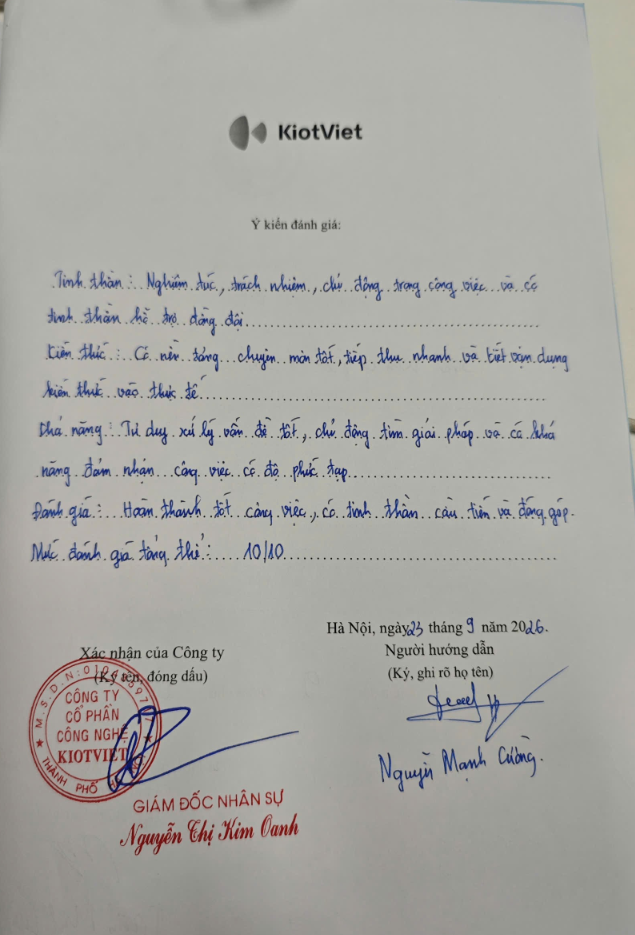
\includegraphics[width=\paperwidth,height=\paperheight]{hinh/danh-gia-cong-ty-cropped.png}
  };
\end{tikzpicture}
\mbox{}
\clearpage

%==================== TRANG DANH GIA CUA GIANG VIEN ====================
\thispagestyle{empty}
\begin{tikzpicture}[remember picture,overlay]
  \node[anchor=east,inner sep=0pt] at (current page.east) {
    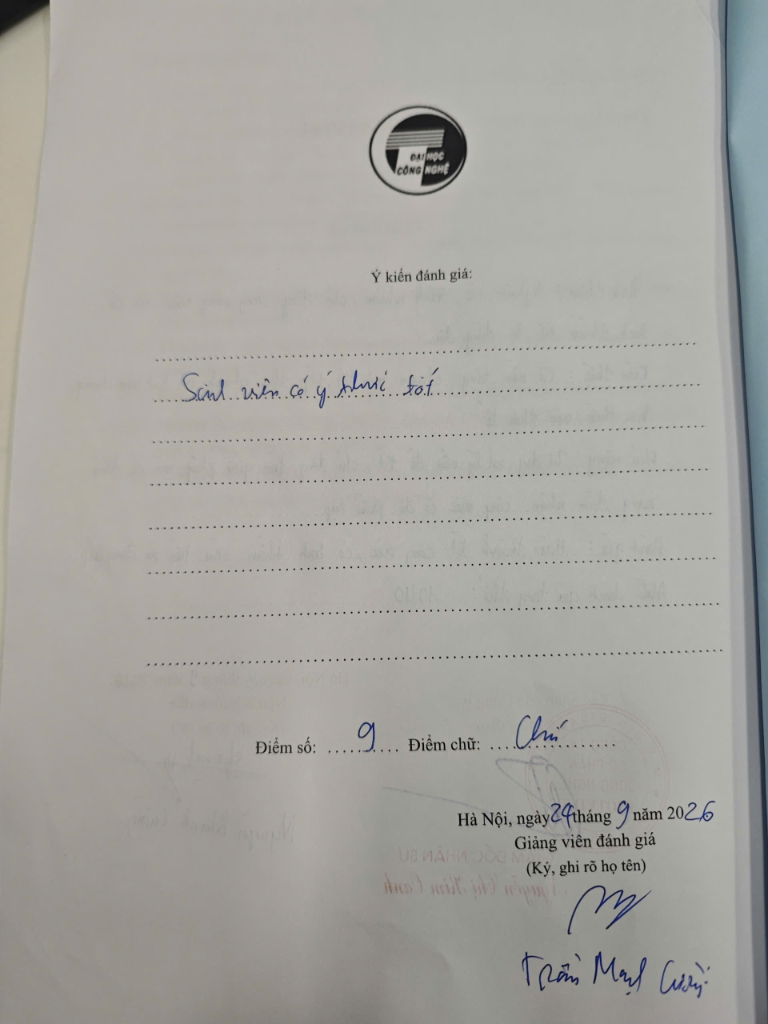
\includegraphics[height=\paperheight,keepaspectratio]{hinh/danh-gia-giang-vien.png}
  };
\end{tikzpicture}
\mbox{}





\end{document}
